\newpage
\section{Интеграл от функции комплексного переменного вдоль пути в $\mathbb{C}$. Его свойства.}


\textbf{Путь} -- параметризованная кривая, возможно с самопересечением (непрерывное отображение $\gamma$ : $[a, b]\subset \mathbb{R} \rightarrow \mathbb{C}$).\\[2mm]
Пусть $\gamma$ -- гладкий путь, то есть $\gamma$ : $z = z(t)$, $t \in J = [\alpha, \beta] \subset \mathbb{R}$, $z(t) \in \mathbb{C}$, $z(J) \subset \mathbb{C}$, функция $f(z)$ определена на $z(J)$ и функция \\ 
$f(z(t))$ : $J \rightarrow \mathbb{C}$ непрерывна (говорят, что $f$ непрерывна на $\gamma$).\\
Число \(\int_{\alpha}^{\beta} f(z(t))z'(t) \,dt\) называют \textbf{интегралом от функции $f$ вдоль пути $\gamma$} и обозначают \(\int_{\gamma} f(z) \, dz\), где $z(t) = x(t) + iy(t)$, $z'(t) = x'(t) + iy'(t)$.\\[2mm]
\textbf{Свойства интеграла:}
\begin{enumerate}
    \item Линейность: \(\int_{\gamma} [af(z) + bf(z)]\, dz\) $=$ $a$\(\int_{\gamma} f(z)\, dz\) $+$ $b$\(\int_{\gamma} f(z)\, dz\);
    \item Ориентированность:
    \begin{figure}[!ht]
    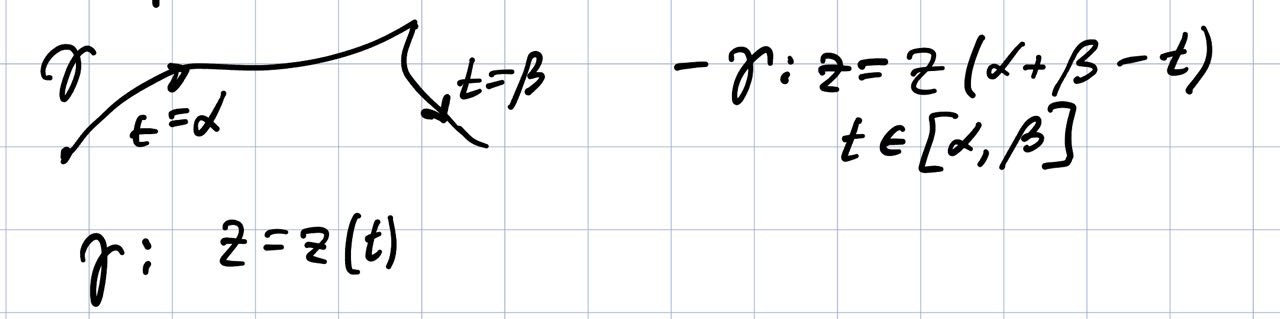
\includegraphics[scale=0.2]{answers/img/pic1.jpg}
    \end{figure}\\
    \(\int_{-\gamma} f(z)\, dz\) $=$ $-$\(\int_{\gamma} f(z)\, dz\);
    \item Аддитивность:\\
    \begin{figure}[!ht]
    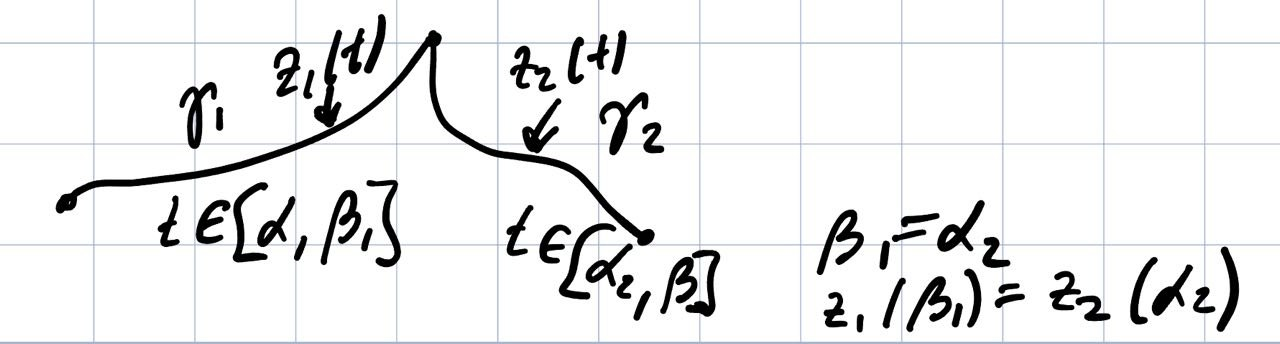
\includegraphics[scale=0.2]{answers/img/pic2.jpg}
    \end{figure}\\
    $\gamma_1 \cup \gamma_2$ : $z = 
    \begin{cases}
        z_1(t), t \in [\alpha, \beta_1];\\
        z_2(t), t \in [\alpha_2, \beta].
    \end{cases}$\\
    \(\int_{\gamma_1 \cup \gamma_2} f\, dz\) $=$ \(\int_{\gamma_1} f\, dz\) $+$ \(\int_{\gamma_2} f\, dz\);
    \item Независимость интеграла от выбора параметризации кривой:\\
    Пусть $\gamma$ : $z = z(t)$, $t \in [\alpha, \beta]$, $\gamma_1$ : $z = z_1(\tau)$ , $\tau \in [\alpha_1, \beta_1]$ -- два непрерывно дифференцируемых пути, $z_1(\tau) = z(t(\tau))$ $\forall \tau \in [\alpha_1, \beta_1]$, где $t = t(\tau)$ : $[\alpha_1, \beta_1] \rightarrow [\alpha, \beta]$ -- непрерывно дифференцируемая возрастающая функция, $f$ непрерывна на $\gamma$.\\
    Тогда \(\int_{\gamma} f\, dz\) $=$ \(\int_{\gamma_1} f\, dz\);
    \item Оценка интеграла:\\
    Если $f$ -- непрерывная функция на кусочно-гладком пути $\gamma$ : $z = z(t)$, $t \in [\alpha, \beta]$, то 
    |\(\int_{\gamma} f\, dz\)| $\leq$ \(\int_{\gamma} |f(z)||z'(t)|\, dt\)\\ 
    ( $|z'(t)|dt = |dz|$ -- дифференциал длины дуги).
\end{enumerate}

\begin{proof}
    \ \\
    4. Независимость интеграла:\\
    $\int\limits_{\gamma}  fdz = \int\limits_{\alpha}^{\beta} f(z(t))z'(t)dt =$\[
    \left | 
    t=t(\tau), \ 
    dt=t'(\tau)d\tau, \ 
    \frac{dz(t(\tau))}{d\tau} = \frac{dt}{d\tau}\frac{dz(t(\tau))}{dt}
    \right |    
    \]
    $ = \int\limits_{\alpha_1}^{\beta_1} f(z(t(z))) \cdot z'(t(\tau))t'(\tau)d\tau = \int\limits_{\alpha_1}^{\beta_1} f(z_1(\tau))z'(\tau)d\tau = \int\limits_{\gamma_1}dz$\\
    5. Оценка интеграла:\\
    Пусть $I=\int\limits_{\gamma} fdz \in \mathbb{C} = |I|\cdot \exp^{i\theta}$\\
    $|I|=\exp^{-i\theta}\cdot I = \int\exp^{-i\theta}f[z(t)]z'(t)dt$\\
    Обозначим $g(t) = \exp^{-i\theta}f[z(t)]z'(t)$.\\
    Тогда $|I| = \int\limits_{\alpha}^{\beta} Re \, g(t)dt+i\int\limits_{\alpha}^{\beta} Im \,g(t)dt\leq \int\limits_{\alpha}^{\beta}|g(t)|dt=\int\limits_{\alpha}^{\beta}|\exp^{-i\theta}|\cdot |f(z(t))|\cdot |z'(t)|dt$
\end{proof}
